\documentclass[11pt]{article}
\usepackage[top=1in, bottom=1in, left=1in, right=1in]{geometry}
\usepackage{tikz}
\usetikzlibrary{shapes,arrows,matrix,patterns,positioning}
\usepackage{color}
%\usepackage[parfill]{parskip}
\usepackage{graphicx}
\usepackage{algorithmic}
\usepackage{amssymb}
\usepackage{epstopdf}
\usepackage[ruled]{algorithm2e}
\usepackage{float}
\usepackage{amsmath,amsthm,bm,color,epsfig,enumerate,caption}
\usepackage{hyperref}
\usepackage{booktabs}
\usepackage{multirow}
\usepackage{array}

%\linespread{2}

% to highlight the latest changes
\newcommand{\alert}[1]{\textcolor{red}{#1}}

\newcommand{\hz}[1]{{\textbf{HZ: #1}}}
\newcommand{\yl}[1]{\textcolor{orange}{\textbf{Ryan: #1}}}
\newcommand{\erm}[1]{\textcolor{red}{\textbf{EM: #1}}}
\newtheorem{theorem}{Theorem}[section]
\newtheorem{outline}[theorem]{Outline}
\newtheorem{corollary}[theorem]{Corollary}
\newtheorem{definition}[theorem]{Definition}
\newtheorem{lemma}[theorem]{Lemma}
\newtheorem{proposition}[theorem]{Proposition}
\newtheorem{algo}[theorem]{Algorithm}
\newtheorem{remark}[theorem]{Remark}
\renewcommand{\appendix}[1]{
\section*{Appendix: #1}
}
\newcommand{\norm}[1]{\left\lVert#1\right\rVert}
%\newcommand{\herm}[1]{(#1)^*}
%\renewcommand{\L}{\mathcal{L}}
%\renewcommand{\O}{\mathcal{O}}
\renewcommand{\O}{O}
%\newcommand{\K}{\mathcal{K}}
%\newcommand{\F}{\mathcal{F}}
\newcommand{\bbZ}{\mathbb{Z}}
\newcommand{\bbF}{\mathbb{F}}
\newcommand{\bbC}{\mathbb{C}}
\newcommand{\bbR}{\mathbb{R}}
\newcommand{\rID}{{\it rID}}
\newcommand{\cID}{{\it cID}}
\newcommand{\blue}{\textcolor{blue}}

\makeatletter
\newcommand*{\extendadd}{
  \mathbin{
    \mathpalette\extend@add{}
  }
}
\newcommand*{\extend@add}[2]{
  \ooalign{
    $\m@th#1\leftrightarrow$%
    \vphantom{$\m@th#1\updownarrow$}
    \cr
    \hfil$\m@th#1\updownarrow$\hfil
  }
}
\makeatother

\begin{document}

\title{Numerical Comparison Summary}
%\author{Qiyuan Pang \\ Tsinghua University, China\\  \href{mailto:ppangqqyz@foxmail.com}{ppangqqyz@foxmail.com} 
%   \and Kenneth L. Ho \\ San Francisco, CA, USA\\ \href{mailto:klho@alumni.caltech.edu}{klho@alumni.caltech.edu}
%     \and Haizhao Yang \\ Department of Mathematics\\ National University of Singapore, Singapore\\ \href{mailto:haizhao@nus.edu.sg}{haizhao@nus.edu.sg} }
\author{Qiyuan Pang}

\maketitle

According to the preprint, we solve $K x = b$ by solving 
\begin{equation*}
\hat{K}^{*}\hat{K}x = \hat{K}^{*}b,
\end{equation*}
preconditioned with and without $\hat{G} = (\hat{K}^{*}\hat{K})^{-1}$. The following quantities are used in the rest of the section to
evaluate the performance of the preconditioner:

\begin{itemize}
\item N: problem size;
\item $e_{a}$: the relative error set for the butterfly approximation $\hat{K}$ of $K$;
\item $\epsilon$: the fixed tolerance set in HIF/HQR;
\item $e_{f}$: forward error of a factorization (HIF/HQR) (e.g., $\hat{A}$ factorizes $A$, then $e_{f} = \|\hat{A}x-Ax\|/\|Ax\|$);
\item $e_{h}$: the accuracy of HODLR construction using the peeling algorithm.
\item $r_{h}$: the maximum rank recorded from the HODLR construction above.
\item $e_{s}$: the relative error of the approximation $\hat{G}\hat{K}^{*}$ of $K^{-1}$, defined as $\|\hat{G}\hat{K}^{*}b - x\|/\|x\|$ where $x$ is a random vector and $b = Kx$;
\item $n_{i}$: the number of iterations used in PCG until covergence;
\item $e$: the relative error of the solution returned by PCG.
\end{itemize}

Among all experiments below, the stopping criteria set for PCG is tolerance $1e-8$.

\textbf{Examples (1D).} We begin with an example of 1D discrete FIO of the form
\begin{equation*}
u(x) = \int\limits_{\mathbb{R}}a(x)e^{2\pi i \Phi(x, \xi)}\hat{f}(\xi) d\xi
\end{equation*}


There are five 1D kernels to test here, as follows:

\begin{equation}
a = 1, \Phi(x,\xi) = x\cdot\xi + c(x)|\xi|, c(x) = (2+\sin(2\pi x))/8,
\end{equation}

\begin{equation}
a = 1, \Phi(x,\xi) = x\cdot\xi + c(x)\xi, c(x) = (2+\sin(2\pi x))/6.5,
\end{equation}

\begin{equation}
a = \sum\limits_{k=0}^{n_{k}} e^{-\frac{(x-x_{k})^2 + (\xi-\xi_{k})^2}{\sigma^2}}, \sigma = 0.05, \Phi(x,\xi) = x\cdot\xi + c(x)|\xi|, c(x) = (2+\sin(2\pi x))/8,
\end{equation}

\begin{equation}
a = \sum\limits_{k=0}^{n_{k}} e^{-\frac{(x-x_{k})^2 + (\xi-\xi_{k})^2}{\sigma^2}}, \sigma = 0.1, \Phi(x,\xi) = x\cdot\xi + c(x)|\xi|, c(x) = (2+\sin(2\pi x))/8,
\end{equation}

\begin{equation}
a = \sum\limits_{k=0}^{n_{k}} e^{-\frac{(x-x_{k})^2 + (\xi-\xi_{k})^2}{\sigma^2}}, \sigma = 0.05, \Phi(x,\xi) = x\cdot\xi + c(x)|\xi|, c(x) = (2+\sin(2\pi x))/7,
\end{equation}


\textbf{Note that the amplitude function $a$ in (3), (4), and (5) are as the same as that in Example 2 in Lexing's preprint. Here we skip the exact formula of $a$.}

Discretizing $x$ and $\xi$ on $[0,1)$ and $[-N/2, N/2)$ with $N$ points,
\begin{equation*}
x_{i} = (i-1)/N, \xi_{j} = j-1-N/2.
\end{equation*}
leads to the discrete system $u = Kf$.



Table \ref{1d-k1} summarizes the results for 1D kernel (1).
Table \ref{1d-k2} summarizes the results for 1D kernel (2).
Table \ref{1d-k3} summarizes the results for 1D kernel (3).
Table \ref{1d-k4} summarizes the results for 1D kernel (4).
Table \ref{1d-k5} summarizes the results for 1D kernel (5).

\textbf{Scaling.} See Figure \ref{fig} for time scaling of the algorithms involved. 


%\begin{table}[!htbp]
%\centering
%\begin{tabular}{|c|c|c|c|c|c|}
%\hline
%N & Kernel 1 & Kernel 2 & Kernel 3 & Kernel 4 & Kernel 5\\ 
%
%
%\end{tabular}
%
%\caption{Numerical comparison between HIF and HQR. We solve 1D kernel (1) equation by using the approximate inverse $\hat{G}\hat{K}^{*}$ as preconditioners for PCG with tolerance $1e-8$. We also solve the equation by pure CG without any preconditioners and set the maximum iteration number to be 200.}
%\label{1d-cond}
%\end{table}


\begin{figure}[ht!]
  \begin{center}
    \begin{tabular}{cc}
      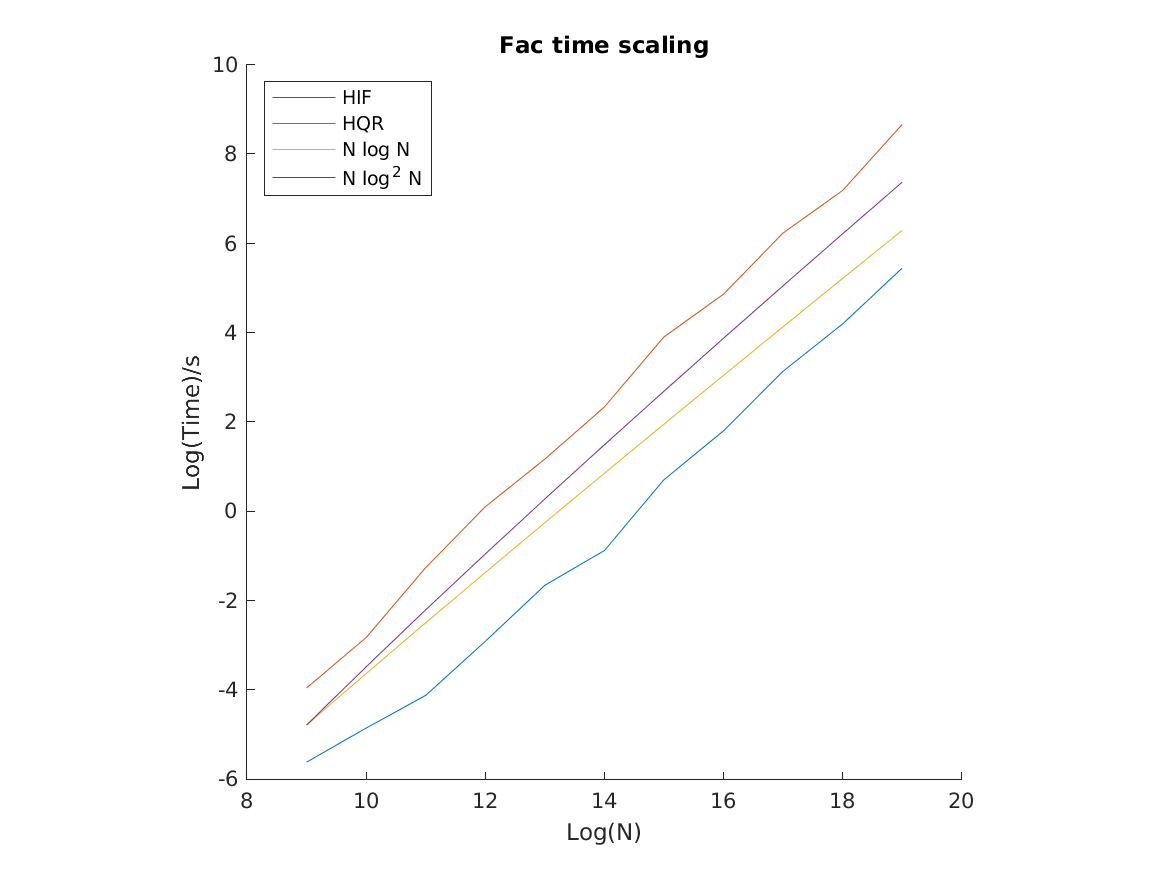
\includegraphics[height=2.7in]{../../scaling/fio/factime_fun_FIO.png}&
      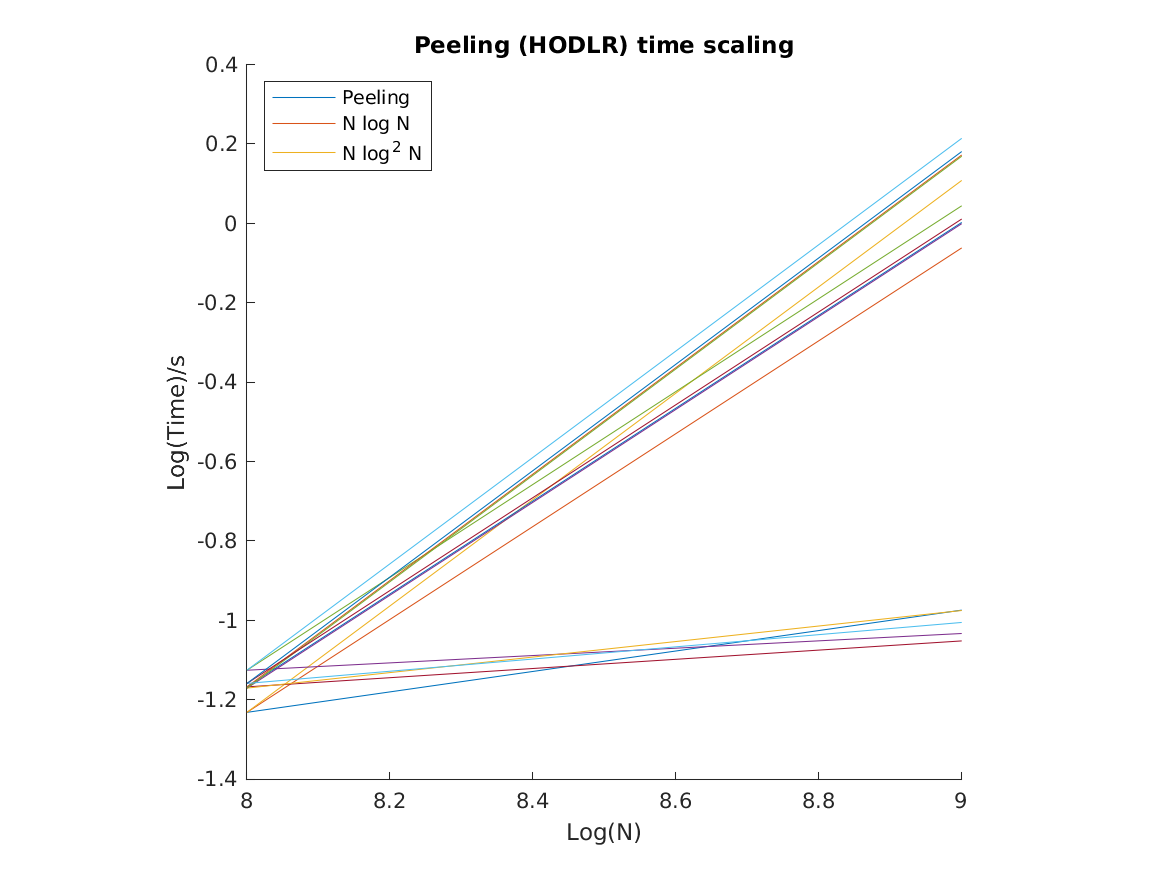
\includegraphics[height=2.7in]{../../scaling/fio/hodlrtime_fun_FIO.png}\\
      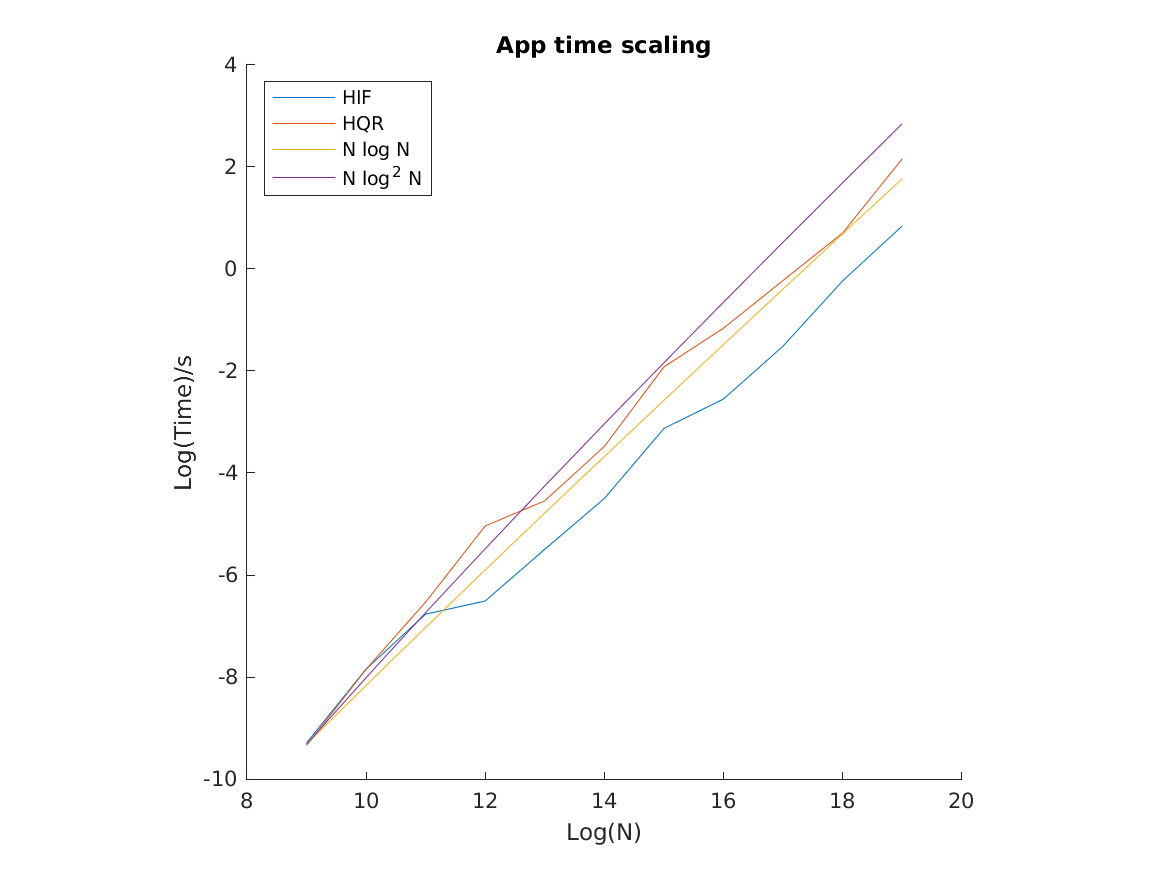
\includegraphics[height=2.7in]{../../scaling/fio/apptime_fun_FIO.png}&   
      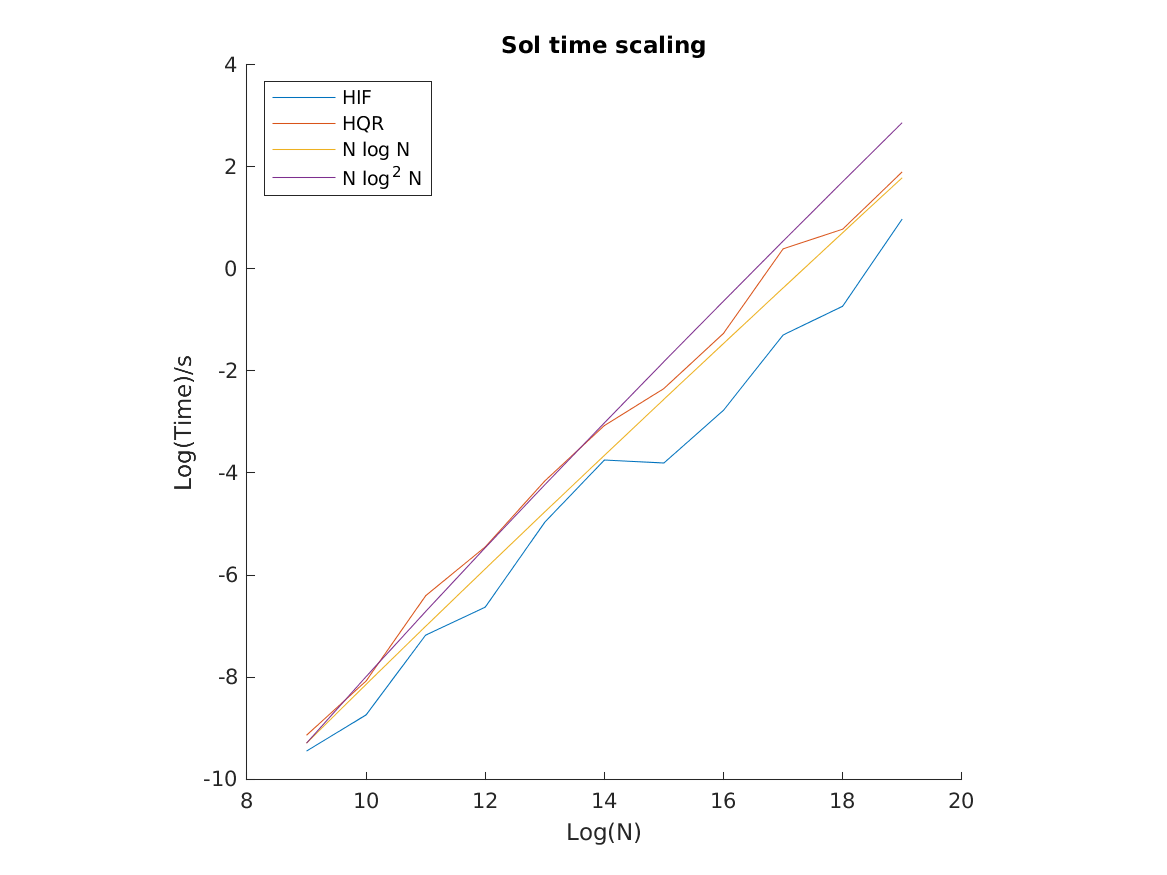
\includegraphics[height=2.7in]{../../scaling/fio/soltime_fun_FIO.png}
    \end{tabular}
  \end{center}
\caption{The upper left, upper right, lower left, and lower right plot the time scaling of HIF/HQR factorization, peeling algorithm, application of HIF/HQR factorization, and backward application of HIF/HQR factorization, respectively. }
\label{fig}
\end{figure}


\begin{table}[!htbp]
\centering
\begin{tabular}{|c|c|c|c|c|c|c|c|c|c|c|c|c|c|c|}
\hline
\multicolumn{1}{c|}{} & \multicolumn{1}{c|}{$\hat{K} \approx K$} & \multicolumn{2}{c|}{$HODLR$} & \multicolumn{1}{c|}{} &\multicolumn{4}{c|}{HIF} & \multicolumn{4}{c|}{HQR} & \multicolumn{2}{c|}{CG} \\
\hline
N & $e_{a}$ & $e_{h}$ & $r_{h}$ & $\epsilon$ & $e_{f}$ & $e_{s}$ & $n_{i}$ & $e$ & $e_{f}$  & $e_{s}$ & $n_{i}$ & $e$ &  $n_{i}$ & $e$ \\ 
\hline
$2^{8}$ & 9e-16 & 1e-05 & 10 & 1e-3 & 1e-05 & 2e-05 & 2 & 1e-09 & 4e-04 & 2e-04 & 3 & 1e-09 & 26 & 8e-09\\
~ & ~ & 1e-06 & 14 & 1e-4 & 2e-06 & 3e-06 & 2 & 3e-11 & 3e-05 & 2e-05 & 2 & 1e-09 & 26 & 8e-09\\
\hline
$2^{9}$ & 3e-09 & 2e-05 & 10 & 1e-3 & 2e-05 & 2e-05 & 2 & 3e-09 & 4e-04 & 2e-04 & 3 & 2e-10 & 27 & 7e-09\\
~ & ~ & 1e-06 & 14 & 1e-4 & 3e-06 & 3e-06 & 2 & 7e-11 & 3e-05 & 3e-05 & 2 & 1e-09 & 27 & 7e-09\\
\hline
$2^{10}$ & 2e-09 & 2e-05 & 10 & 1e-3 & 3e-05 & 3e-05 & 2 & 5e-09 & 3e-04 & 2e-04 & 3 & 1e-10 & 27 & 9e-09\\
~ & ~ & 1e-06 & 14 & 1e-4 & 3e-06 & 4e-06 & 2 & 8e-11 & 3e-05 & 2e-05 & 2 & 1e-09 & 27 & 9e-09\\
\hline
$2^{11}$ & 6e-09 & 2e-05 & 10 & 1e-3 & 3e-05 & 3e-05 & 2 & 8e-09 & 3e-04 & 3e-04 & 3 & 1e-10 & 27 & 1e-08\\
~ & ~ & 2e-06 & 14 & 1e-4 & 4e-06 & 4e-06 & 2 & 8e-11 & 3e-05 & 2e-05 & 2 & 1e-09 & 27 & 1e-08\\
\hline
$2^{12}$ & 4e-09 & 2e-05 & 10 & 1e-3 & 3e-05 & 3e-05 & 2 & 9e-09 & 3e-04 & 2e-04 & 3 & 1e-10 & 28 & 5e-09\\
~ & ~ & 2e-06 & 14 & 1e-4 & 4e-06 & 4e-06 & 2 & 9e-11 & 3e-05 & 2e-05 & 2 & 1e-09 & 28 & 5e-09\\
\hline
$2^{13}$ & 9e-09 & 2e-05 & 10 & 1e-3 & 4e-05 & 3e-05 & 2 & 9e-09 & 3e-04 & 2e-04 & 3 & 1e-10 & 27 & 1e-08\\
~ & ~ & 2e-06 & 14 & 1e-4 & 3e-06 & 3e-06 & 2 & 6e-11 & 3e-05 & 2e-05 & 2 & 1e-09 & 28 & 5e-09\\
\hline
$2^{14}$ & 6e-09 & 2e-05 & 10 & 1e-3 & 6e-05 & 4e-05 & 3 & 3e-11 & 3e-04 & 2e-04 & 3 & 1e-10 & 27 & 1e-08\\
~ & ~ & 2e-06 & 14 & 1e-4 & 3e-06 & 3e-06 & 2 & 8e-11 & 3e-05 & 2e-05 & 2 & 1e-09 & 28 & 5e-09\\
\hline
$2^{15}$ & 1e-08 & 2e-05 & 10 & 1e-3 & 8e-05 & 6e-05 & 3 & 9e-11 & 3e-04 & 2e-04 & 3 & 1e-10 & 28 & 5e-09\\
~ & ~ & 2e-06 & 14 & 1e-4 & 7e-06 & 7e-06 & 2 & 6e-10 & 3e-05 & 2e-05 & 2 & 1e-09 & 28 & 5e-09\\
\hline
$2^{16}$ & 6e-09 & 2e-05 & 10 & 1e-3 & 7e-05 & 6e-05 & 3 & 5e-11 & 3e-04 & 2e-04 & 3 & 1e-10 & 27 & 1e-08\\
~ & ~ & 2e-06 & 14 & 1e-4 & 1e-05 & 1e-05 & 2 & 1e-09 & 3e-05 & 2e-05 & 2 & 1e-09 & 27 & 1e-08\\
\hline
$2^{17}$ & 1e-08 & 2e-05 & 10 & 1e-3 & 1e-04 & 7e-05 & 3 & 8e-11 & 3e-04 & 2e-04 & 3 & 1e-10 & 27 & 9e-09\\
~ & ~ & 2e-06 & 14 & 1e-4 & 1e-05 & 1e-05 & 2 & 1e-09 & 3e-05 & 2e-05 & 2 & 1e-09 & 27 & 1e-08\\
\hline
$2^{18}$ & 7e-09 & 2e-05 & 10 & 1e-3 & 1e-04 & 7e-05 & 3 & 7e-11 & 3e-04 & 2e-04 & 3 & 1e-10 & 27 & 5e-09\\
~ & ~ & 2e-06 & 14 & 1e-4 & 2e-05 & 2e-05 & 2 & 2e-09 & 3e-05 & 2e-05 & 2 & 1e-09 & 27 & 7e-09\\
\hline
$2^{19}$ & 1e-08 & 2e-05 & 10 & 1e-3 & 1e-04 & 1e-04 & 3 & 1e-10 & 3e-04 & 2e-04 & 3 & 1e-10 & 27 & 8e-09\\
~ & ~ & 2e-06 & 14 & 1e-4 & 1e-05 & 2e-05 & 2 & 1e-09 & 3e-05 & 2e-05 & 2 & 1e-09 & 27 & 6e-09\\


\end{tabular}

\caption{Numerical comparison between HIF and HQR. We solve 1D kernel (1) equation by using the approximate inverse $\hat{G}\hat{K}^{*}$ as preconditioners for PCG with tolerance $1e-8$. We also solve the equation by pure CG without any preconditioners and set the maximum iteration number to be 200.}
\label{1d-k1}
\end{table}


\begin{table}[!htbp]
\centering
\begin{tabular}{|c|c|c|c|c|c|c|c|c|c|c|c|c|c|c|}
\hline
\multicolumn{1}{c|}{} & \multicolumn{1}{c|}{$\hat{K} \approx K$} & \multicolumn{2}{c|}{$HODLR$} & \multicolumn{1}{c|}{} &\multicolumn{4}{c|}{HIF} & \multicolumn{4}{c|}{HQR} & \multicolumn{2}{c|}{Pure CG} \\
\hline
N & $e_{a}$ & $e_{h}$ & $r_{h}$ & $\epsilon$ & $e_{f}$ & $e_{s}$ & $n_{i}$ & $e$ & $e_{f}$  & $e_{s}$ & $n_{i}$ & $e$ &  $n_{i}$ & $e$ \\ 
\hline
$2^{8}$ & 9e-16 & 3e-05 & 17 & 1e-3 & 1e-04 & 2e-04 & 3 & 9e-11 & 3e-04 & 4e-04 & 3 & 7e-10 & 32 & 9e-09\\
~ & ~ & 3e-06 & 19 & 1e-4 & 1e-05 & 1e-05 & 2 & 8e-10 & 3e-05 & 3e-05 & 2 & 3e-09 & 32 & 9e-09\\
\hline
$2^{9}$ & 2e-09 & 4e-05 & 18 & 1e-3 & 3e-04 & 2e-04 & 3 & 2e-10 & 3e-04 & 3e-04 & 3 & 5e-10 & 38 & 1e-08\\
~ & ~ & 7e-06 & 20 & 1e-4 & 3e-05 & 2e-05 & 2 & 3e-09 & 2e-05 & 3e-05 & 2 & 5e-09 & 38 & 1e-08\\
\hline
$2^{10}$ & 2e-09 & 5e-05 & 19 & 1e-3 & 6e-04 & 3e-04 & 3 & 1e-09 & 4e-04 & 3e-04 & 3 & 1e-09 & 45 & 9e-09\\
~ & ~ & 2e-05 & 20 & 1e-4 & 4e-05 & 3e-05 & 3 & 3e-12 & 3e-05 & 3e-05 & 2 & 1e-08 & 45 & 1e-08\\
\hline
$2^{11}$ & 8e-09 & 4e-05 & 20 & 1e-3 & 4e-04 & 3e-04 & 3 & 1e-09 & 5e-04 & 3e-04 & 3 & 3e-09 & 54 & 1e-08\\
~ & ~ & 2e-05 & 20 & 1e-4 & 6e-05 & 5e-05 & 3 & 2e-11 & 5e-05 & 5e-05 & 3 & 1e-11 & 54 & 9e-09\\
\hline
$2^{12}$ & 4e-09 & 5e-05 & 20 & 1e-3 & 7e-04 & 4e-04 & 3 & 9e-09 & 3e-04 & 4e-04 & 3 & 1e-09 & 62 & 1e-08\\
~ & ~ & 2e-05 & 20 & 1e-4 & 8e-05 & 6e-05 & 3 & 8e-11 & 4e-05 & 4e-05 & 3 & 8e-11 & 62 & 1e-08\\
\hline
$2^{13}$ & 1e-08 & 4e-05 & 20 & 1e-3 & 9e-04 & 4e-04 & 3 & 6e-09 & 4e-04 & 3e-04 & 3 & 9e-10 & 69 & 1e-08\\
~ & ~ & 1e-05 & 20 & 1e-4 & 6e-05 & 6e-05 & 3 & 3e-11 & 3e-05 & 3e-05 & 3 & 2e-11 & 69 & 1e-08\\
\hline
$2^{14}$ & 5e-09 & 4e-05 & 20 & 1e-3 & 1e-03 & 4e-04 & 4 & 6e-11 & 4e-04 & 3e-04 & 3 & 1e-09 & 75 & 9e-09\\
~ & ~ & 2e-05 & 20 & 1e-4 & 8e-05 & 6e-05 & 3 & 4e-11 & 4e-05 & 3e-05 & 3 & 3e-11 & 76 & 7e-09\\
\hline
$2^{15}$ & 1e-08 & 4e-05 & 20 & 1e-3 & 9e-04 & 4e-04 & 4 & 5e-11 & 4e-04 & 3e-04 & 3 & 1e-09 & 76 & 1e-08\\
~ & ~ & 1e-05 & 20 & 1e-4 & 8e-05 & 7e-05 & 3 & 3e-11 & 3e-05 & 3e-05 & 3 & 2e-11 & 76 & 1e-08\\
\hline
$2^{16}$ & 7e-09 & 4e-05 & 20 & 1e-3 & 1e-03 & 4e-04 & 4 & 1e-10 & 4e-04 & 3e-04 & 3 & 9e-10 & 77 & 8e-09\\
~ & ~ & 1e-05 & 20 & 1e-4 & 1e-04 & 7e-05 & 3 & 5e-11 & 3e-05 & 2e-05 & 3 & 3e-11 & 77 & 8e-09\\
\hline
$2^{17}$ & 2e-08 & 4e-05 & 20 & 1e-3 & 1e-03 & 4e-04 & 4 & 5e-11 & 4e-04 & 3e-04 & 3 & 9e-10 & 77 & 8e-09\\
~ & ~ & 8e-06 & 20 & 1e-4 & 1e-04 & 8e-05 & 3 & 4e-11 & 3e-05 & 2e-05 & 2 & 2e-08 & 77 & 8e-09\\
\hline
$2^{18}$ & 8e-09 & 4e-05 & 20 & 1e-3 & 1e-03 & 4e-04 & 4 & 9e-11 & 4e-04 & 3e-04 & 3 & 1e-09 & 77 & 8e-09\\
~ & ~ & 9e-06 & 20 & 1e-4 & 1e-04 & 8e-05 & 3 & 5e-11 & 3e-05 & 2e-05 & 2 & 1e-08 & 77 & 8e-09\\
\hline
$2^{19}$ & 2e-08 & 4e-05 & 20 & 1e-3 & 1e-03 & 4e-04 & 4 & 1e-10 & 4e-04 & 3e-04 & 3 & 9e-10 & 77 & 8e-09\\
~ & ~ & 7e-06 & 20 & 1e-4 & 1e-04 & 9e-05 & 3 & 8e-11 & 3e-05 & 2e-05 & 2 & 1e-08 & 77 & 8e-09\\



\end{tabular}

\caption{Numerical comparison between HIF and HQR. We solve 1D kernel (2) equation by using the approximate inverse $\hat{G}\hat{K}^{*}$ as preconditioners for PCG with tolerance $1e-8$. We also solve the equation by pure CG without any preconditioners and set the maximum iteration number to be 200.}
\label{1d-k2}
\end{table}


\begin{table}[!htbp]
\centering
\begin{tabular}{|c|c|c|c|c|c|c|c|c|c|c|c|c|c|c|}
\hline
\multicolumn{1}{c|}{} & \multicolumn{1}{c|}{$\hat{K} \approx K$} & \multicolumn{2}{c|}{$HODLR$} & \multicolumn{1}{c|}{} &\multicolumn{4}{c|}{HIF} & \multicolumn{4}{c|}{HQR} & \multicolumn{2}{c|}{Pure CG} \\
\hline
N & $e_{a}$ & $e_{h}$ & $r_{h}$ & $\epsilon$ & $e_{f}$ & $e_{s}$ & $n_{i}$ & $e$ & $e_{f}$  & $e_{s}$ & $n_{i}$ & $e$ &  $n_{i}$ & $e$ \\ 
\hline
$2^{8}$ & 1e-15 & 7e-06 & 11 & 1e-3 & 5e-05 & 5e-04 & 3 & 8e-08 & 2e-04 & 2e-03 & 5 & 4e-07 & 187 & 1e-02\\
~ & ~ & 1e-06 & 14 & 1e-4 & 5e-06 & 7e-05 & 2 & 1e-07 & 2e-05 & 5e-04 & 3 & 7e-06 & 187 & 1e-02\\
\hline
$2^{9}$ & 3e-09 & 1e-05 & 10 & 1e-3 & 2e-05 & 5e-04 & 3 & 7e-08 & 1e-04 & 3e-03 & 5 & 1e-07 & 200 & 2e-02\\
~ & ~ & 1e-06 & 14 & 1e-4 & 6e-06 & 1e-04 & 2 & 2e-07 & 1e-05 & 7e-05 & 3 & 1e-07 & 200 & 2e-02\\
\hline
$2^{10}$ & 2e-09 & 1e-05 & 10 & 1e-3 & 4e-05 & 5e-04 & 3 & 1e-07 & 3e-04 & 2e-03 & 4 & 9e-07 & 193 & 3e-02\\
~ & ~ & 1e-06 & 13 & 1e-4 & 5e-06 & 1e-04 & 2 & 5e-07 & 1e-05 & 3e-04 & 3 & 2e-07 & 193 & 3e-02\\
\hline
$2^{11}$ & 6e-09 & 1e-05 & 10 & 1e-3 & 5e-05 & 7e-04 & 3 & 1e-07 & 2e-04 & 2e-03 & 5 & 5e-06 & 197 & 5e-02\\
~ & ~ & 1e-06 & 13 & 1e-4 & 5e-06 & 1e-04 & 2 & 4e-07 & 1e-05 & 3e-04 & 3 & 1e-06 & 197 & 5e-02\\
\hline
$2^{12}$ & 4e-09 & 1e-05 & 10 & 1e-3 & 5e-05 & 6e-04 & 3 & 1e-07 & 2e-04 & 2e-03 & 6 & 2e-06 & 196 & 4e-02\\
~ & ~ & 1e-06 & 13 & 1e-4 & 5e-06 & 1e-04 & 2 & 4e-07 & 2e-05 & 2e-04 & 3 & 3e-06 & 196 & 4e-02\\
\hline
$2^{13}$ & 9e-09 & 1e-05 & 10 & 1e-3 & 4e-05 & 6e-04 & 3 & 1e-07 & 2e-04 & 2e-03 & 4 & 5e-06 & 199 & 6e-02\\
~ & ~ & 1e-06 & 13 & 1e-4 & 6e-06 & 1e-04 & 2 & 4e-07 & 2e-05 & 2e-04 & 3 & 3e-06 & 198 & 5e-02\\
\hline
$2^{14}$ & 6e-09 & 1e-05 & 10 & 1e-3 & 5e-05 & 8e-04 & 3 & 1e-06 & 2e-04 & 1e-03 & 4 & 1e-07 & 200 & 5e-02\\
~ & ~ & 1e-06 & 13 & 1e-4 & 5e-06 & 1e-04 & 2 & 6e-07 & 2e-05 & 2e-04 & 3 & 6e-07 & 199 & 5e-02\\
\hline
$2^{15}$ & 9e-09 & 1e-05 & 10 & 1e-3 & 7e-05 & 1e-03 & 4 & 8e-07 & 2e-04 & 1e-03 & 5 & 3e-06 & 200 & 5e-02\\
~ & ~ & 1e-06 & 13 & 1e-4 & 2e-05 & 5e-04 & 3 & 1e-07 & 2e-05 & 2e-04 & 3 & 7e-07 & 200 & 5e-02\\
\hline
$2^{16}$ & 6e-09 & 1e-05 & 10 & 1e-3 & 8e-05 & 1e-03 & 4 & 1e-07 & 2e-04 & 1e-03 & 4 & 4e-06 & 200 & 5e-02\\
~ & ~ & 1e-06 & 13 & 1e-4 & 2e-05 & 5e-04 & 3 & 1e-07 & 2e-05 & 2e-04 & 3 & 2e-06 & 200 & 5e-02\\
\hline
$2^{17}$ & 1e-08 & 1e-05 & 10 & 1e-3 & 9e-05 & 1e-03 & 4 & 7e-07 & 2e-04 & 1e-03 & 6 & 3e-06 & 200 & 5e-02\\
~ & ~ & 1e-06 & 13 & 1e-4 & 2e-05 & 5e-04 & 3 & 1e-07 & 2e-05 & 1e-04 & 3 & 2e-06 & 200 & 5e-02\\
\hline
$2^{18}$ & 8e-09 & 1e-05 & 10 & 1e-3 & 9e-05 & 1e-03 & 4 & 2e-06 & 2e-04 & 1e-03 & 4 & 5e-06 & 200 & 5e-02\\
~ & ~ & 1e-06 & 13 & 1e-4 & 3e-05 & 6e-04 & 3 & 2e-07 & 2e-05 & 1e-04 & 3 & 3e-07 & 200 & 5e-02\\
\hline
$2^{19}$ & 1e-08 & 1e-05 & 10 & 1e-3 & 1e-04 & 1e-03 & 4 & 2e-06 & 2e-04 & 1e-03 & 5 & 2e-06 & 200 & 5e-02\\
~ & ~ & 1e-06 & 13 & 1e-4 & 3e-05 & 6e-04 & 3 & 1e-07 & 2e-05 & 1e-04 & 3 & 1e-07 & 200 & 5e-02\\



\end{tabular}

\caption{Numerical comparison between HIF and HQR. We solve 1D kernel (3) equation by using the approximate inverse $\hat{G}\hat{K}^{*}$ as preconditioners for PCG with tolerance $1e-8$. We also solve the equation by pure CG without any preconditioners and set the maximum iteration number to be 200.}
\label{1d-k3}
\end{table}


\begin{table}[!htbp]
\centering
\begin{tabular}{|c|c|c|c|c|c|c|c|c|c|c|c|c|c|c|}
\hline
\multicolumn{1}{c|}{} & \multicolumn{1}{c|}{$\hat{K} \approx K$} & \multicolumn{2}{c|}{$HODLR$} & \multicolumn{1}{c|}{} &\multicolumn{4}{c|}{HIF} & \multicolumn{4}{c|}{HQR} & \multicolumn{2}{c|}{Pure CG} \\
\hline
N & $e_{a}$ & $e_{h}$ & $r_{h}$ & $\epsilon$ & $e_{f}$ & $e_{s}$ & $n_{i}$ & $e$ & $e_{f}$  & $e_{s}$ & $n_{i}$ & $e$ &  $n_{i}$ & $e$ \\ 
\hline
$2^{8}$ & 1e-15 & 8e-06 & 13 & 1e-3 & 6e-05 & 9e-05 & 3 & 9e-12 & 5e-04 & 4e-04 & 3 & 4e-09 & 106 & 1e-07\\
~ & ~ & 1e-06 & 16 & 1e-4 & 5e-06 & 1e-05 & 2 & 4e-10 & 5e-05 & 5e-05 & 2 & 2e-08 & 106 & 1e-07\\
\hline
$2^{9}$ & 3e-09 & 1e-05 & 13 & 1e-3 & 5e-05 & 8e-05 & 3 & 6e-11 & 4e-04 & 5e-04 & 3 & 3e-09 & 128 & 9e-08\\
~ & ~ & 1e-06 & 17 & 1e-4 & 5e-06 & 9e-06 & 2 & 1e-09 & 3e-05 & 7e-05 & 2 & 4e-08 & 128 & 9e-08\\
\hline
$2^{10}$ & 2e-09 & 1e-05 & 14 & 1e-3 & 6e-05 & 9e-05 & 3 & 6e-11 & 4e-04 & 5e-04 & 3 & 3e-09 & 145 & 1e-07\\
~ & ~ & 1e-06 & 18 & 1e-4 & 5e-06 & 9e-06 & 2 & 7e-10 & 4e-05 & 6e-05 & 3 & 1e-11 & 145 & 1e-07\\
\hline
$2^{11}$ & 6e-09 & 1e-05 & 14 & 1e-3 & 5e-05 & 1e-04 & 3 & 1e-10 & 4e-04 & 5e-04 & 3 & 4e-08 & 158 & 1e-07\\
~ & ~ & 1e-06 & 19 & 1e-4 & 5e-06 & 1e-05 & 2 & 1e-09 & 5e-05 & 5e-05 & 2 & 3e-08 & 158 & 1e-07\\
\hline
$2^{12}$ & 4e-09 & 1e-05 & 15 & 1e-3 & 5e-05 & 1e-04 & 3 & 8e-10 & 4e-04 & 5e-04 & 3 & 5e-09 & 164 & 1e-07\\
~ & ~ & 2e-06 & 19 & 1e-4 & 5e-06 & 1e-05 & 2 & 1e-09 & 4e-05 & 6e-05 & 2 & 1e-08 & 165 & 1e-07\\
\hline
$2^{13}$ & 9e-09 & 1e-05 & 15 & 1e-3 & 7e-05 & 2e-04 & 3 & 1e-09 & 4e-04 & 5e-04 & 3 & 4e-09 & 170 & 1e-07\\
~ & ~ & 2e-06 & 20 & 1e-4 & 1e-05 & 3e-05 & 2 & 1e-08 & 4e-05 & 6e-05 & 2 & 1e-08 & 170 & 1e-07\\
\hline
$2^{14}$ & 6e-09 & 1e-05 & 16 & 1e-3 & 1e-04 & 2e-04 & 3 & 2e-09 & 4e-04 & 5e-04 & 3 & 4e-09 & 171 & 1e-07\\
~ & ~ & 2e-06 & 20 & 1e-4 & 2e-05 & 4e-05 & 2 & 1e-08 & 4e-05 & 5e-05 & 2 & 1e-08 & 170 & 1e-07\\
\hline
$2^{15}$ & 1e-08 & 1e-05 & 16 & 1e-3 & 1e-04 & 3e-04 & 3 & 3e-09 & 4e-04 & 5e-04 & 3 & 4e-09 & 171 & 1e-07\\
~ & ~ & 2e-06 & 20 & 1e-4 & 1e-05 & 3e-05 & 2 & 1e-08 & 4e-05 & 5e-05 & 2 & 1e-08 & 171 & 1e-07\\
\hline
$2^{16}$ & 8e-09 & 1e-05 & 17 & 1e-3 & 1e-04 & 3e-04 & 3 & 7e-09 & 4e-04 & 5e-04 & 3 & 2e-09 & 172 & 1e-07\\
~ & ~ & 2e-06 & 20 & 1e-4 & 2e-05 & 4e-05 & 2 & 1e-08 & 4e-05 & 6e-05 & 2 & 1e-08 & 171 & 1e-07\\
\hline
$2^{17}$ & 1e-08 & 1e-05 & 17 & 1e-3 & 2e-04 & 4e-04 & 4 & 3e-10 & 4e-04 & 5e-04 & 3 & 3e-09 & 171 & 1e-07\\
~ & ~ & 2e-06 & 20 & 1e-4 & 1e-05 & 3e-05 & 2 & 1e-08 & 4e-05 & 5e-05 & 2 & 1e-08 & 172 & 1e-07\\
\hline
$2^{18}$ & 7e-09 & 1e-05 & 18 & 1e-3 & 2e-04 & 4e-04 & 4 & 5e-10 & 4e-04 & 5e-04 & 3 & 3e-09 & 172 & 1e-07\\
~ & ~ & 3e-06 & 20 & 1e-4 & 2e-05 & 5e-05 & 2 & 4e-08 & 4e-05 & 6e-05 & 2 & 3e-08 & 172 & 1e-07\\
\hline
$2^{19}$ & 1e-08 & 1e-05 & 18 & 1e-3 & 2e-04 & 5e-04 & 4 & 4e-09 & 4e-04 & 5e-04 & 3 & 3e-09 & 172 & 1e-07\\
~ & ~ & 3e-06 & 20 & 1e-4 & 1e-05 & 3e-05 & 2 & 3e-08 & 4e-05 & 5e-05 & 2 & 3e-08 & 172 & 1e-07\\



\end{tabular}

\caption{Numerical comparison between HIF and HQR. We solve 1D kernel (4) equation by using the approximate inverse $\hat{G}\hat{K}^{*}$ as preconditioners for PCG with tolerance $1e-8$. We also solve the equation by pure CG without any preconditioners and set the maximum iteration number to be 200.}
\label{1d-k4}
\end{table}



\begin{table}[!htbp]
\centering
\begin{tabular}{|c|c|c|c|c|c|c|c|c|c|c|c|c|c|c|}
\hline
\multicolumn{1}{c|}{} & \multicolumn{1}{c|}{$\hat{K} \approx K$} & \multicolumn{2}{c|}{$HODLR$} & \multicolumn{1}{c|}{} &\multicolumn{4}{c|}{HIF} & \multicolumn{4}{c|}{HQR} & \multicolumn{2}{c|}{Pure CG} \\
\hline
N & $e_{a}$ & $e_{h}$ & $r_{h}$ & $\epsilon$ & $e_{f}$ & $e_{s}$ & $n_{i}$ & $e$ & $e_{f}$  & $e_{s}$ & $n_{i}$ & $e$ &  $n_{i}$ & $e$ \\ 
\hline
$2^{8}$ & 9e-16 & 2e-05 & 14 & 1e-3 & 1e-04 & 1e-03 & 3 & 2e-06 & 5e-04 & 2e-02 & 186 & 1e-03 & 193 & 2e-02\\
~ & ~ & 1e-06 & 17 & 1e-4 & 1e-05 & 2e-04 & 3 & 2e-08 & 4e-05 & 2e-04 & 3 & 3e-07 & 193 & 2e-02\\
\hline
$2^{9}$ & 4e-09 & 2e-05 & 14 & 1e-3 & 1e-04 & 1e-03 & 3 & 9e-07 & 3e-04 & 4e-03 & 11 & 8e-06 & 185 & 4e-02\\
~ & ~ & 1e-06 & 18 & 1e-4 & 2e-05 & 4e-04 & 3 & 1e-08 & 8e-05 & 1e-03 & 4 & 1e-07 & 185 & 4e-02\\
\hline
$2^{10}$ & 3e-09 & 2e-05 & 14 & 1e-3 & 1e-04 & 3e-03 & 4 & 3e-07 & 6e-04 & 3e-03 & 31 & 5e-06 & 200 & 4e-02\\
~ & ~ & 2e-06 & 17 & 1e-4 & 2e-05 & 4e-04 & 3 & 3e-08 & 5e-05 & 2e-04 & 3 & 2e-06 & 200 & 4e-02\\
\hline
$2^{11}$ & 7e-09 & 3e-05 & 14 & 1e-3 & 2e-04 & 4e-03 & 4 & 1e-06 & 5e-04 & 4e-03 & 13 & 1e-05 & 200 & 7e-02\\
~ & ~ & 2e-06 & 17 & 1e-4 & 1e-05 & 4e-04 & 3 & 2e-08 & 6e-05 & 4e-04 & 3 & 2e-06 & 200 & 7e-02\\
\hline
$2^{12}$ & 6e-09 & 2e-05 & 14 & 1e-3 & 3e-04 & 4e-03 & 5 & 1e-07 & 4e-04 & 4e-03 & 10 & 5e-06 & 196 & 7e-02\\
~ & ~ & 2e-06 & 17 & 1e-4 & 2e-05 & 3e-04 & 3 & 5e-08 & 6e-05 & 5e-04 & 3 & 3e-06 & 198 & 6e-02\\
\hline
$2^{13}$ & 9e-09 & 2e-05 & 14 & 1e-3 & 2e-04 & 5e-03 & 5 & 1e-06 & 5e-04 & 2e-03 & 109 & 4e-05 & 200 & 8e-02\\
~ & ~ & 2e-06 & 17 & 1e-4 & 3e-05 & 8e-04 & 3 & 5e-07 & 6e-05 & 2e-04 & 3 & 3e-07 & 200 & 7e-02\\
\hline
$2^{14}$ & 6e-09 & 2e-05 & 14 & 1e-3 & 3e-04 & 5e-03 & 5 & 1e-06 & 4e-04 & 2e-03 & 6 & 2e-06 & 200 & 7e-02\\
~ & ~ & 2e-06 & 17 & 1e-4 & 4e-05 & 8e-04 & 3 & 4e-07 & 5e-05 & 3e-04 & 3 & 1e-06 & 198 & 8e-02\\
\hline
$2^{15}$ & 1e-08 & 2e-05 & 14 & 1e-3 & 3e-04 & 7e-03 & 6 & 7e-07 & 5e-04 & 2e-03 & 11 & 1e-05 & 197 & 8e-02\\
~ & ~ & 2e-06 & 17 & 1e-4 & 4e-05 & 9e-04 & 3 & 4e-07 & 5e-05 & 2e-04 & 3 & 7e-07 & 198 & 8e-02\\
\hline
$2^{16}$ & 6e-09 & 2e-05 & 14 & 1e-3 & 3e-04 & 6e-03 & 6 & 1e-06 & 5e-04 & 1e-03 & 4 & 8e-06 & 197 & 9e-02\\
~ & ~ & 2e-06 & 17 & 1e-4 & 5e-05 & 1e-03 & 3 & 7e-07 & 5e-05 & 3e-04 & 3 & 4e-08 & 200 & 8e-02\\
\hline
$2^{17}$ & 1e-08 & 2e-05 & 14 & 1e-3 & 3e-04 & 7e-03 & 6 & 5e-07 & 5e-04 & 1e-03 & 6 & 3e-06 & 200 & 9e-02\\
~ & ~ & 2e-06 & 17 & 1e-4 & 5e-05 & 9e-04 & 3 & 6e-07 & 5e-05 & 2e-04 & 3 & 7e-07 & 200 & 9e-02\\
\hline
$2^{18}$ & 8e-09 & 2e-05 & 14 & 1e-3 & 3e-04 & 7e-03 & 6 & 1e-06 & 5e-04 & 2e-03 & 5 & 6e-06 & 200 & 8e-02\\
~ & ~ & 2e-06 & 17 & 1e-4 & 6e-05 & 1e-03 & 3 & 8e-07 & 5e-05 & 2e-04 & 3 & 9e-07 & 200 & 9e-02\\
\hline
$2^{19}$ & 1e-08 & 2e-05 & 14 & 1e-3 & 3e-04 & 6e-03 & 6 & 2e-06 & 5e-04 & 1e-03 & 6 & 3e-06 & 200 & 9e-02\\
~ & ~ & 2e-06 & 17 & 1e-4 & 6e-05 & 1e-03 & 3 & 7e-07 & 5e-05 & 2e-04 & 4 & 2e-07 & 200 & 9e-02\\



\end{tabular}

\caption{Numerical comparison between HIF and HQR. We solve 1D kernel (5) equation by using the approximate inverse $\hat{G}\hat{K}^{*}$ as preconditioners for PCG with tolerance $1e-8$. We also solve the equation by pure CG without any preconditioners and set the maximum iteration number to be 200.}
\label{1d-k5}
\end{table}



\bibliographystyle{unsrt} 
\bibliography{ref}

\end{document}

